% Slides for talk on hydrogen fuel cells
% given in the department on October 27, 2003.
% 
% The original slides were in Prosper.  This file contains the
% translation of the original slides to Beamer.% 
% Rouben Rostamian <rostamian@umbc.edu>
% August 31, 2004

\documentclass[10pt]{beamer}
%\usetheme{umbc4}
\usetheme{Boadilla}
\useinnertheme{umbcboxes}
\setbeamercolor{umbcboxes}{bg=violet!15,fg=black}
\def\newblock{\hskip .11em plus .33em minus .07em}

\setbeamertemplate{navigation symbols}{}

\usepackage{rotating} % for defining \schwa
\usepackage{amsmath}
\usepackage{subfigure}
\usepackage{bm}
\usepackage{natbib}
\usepackage{hyperref}
\usepackage{soul}
\usepackage{tikz}
\usetikzlibrary{shapes.geometric, arrows}
\usepackage{etex}
\usepackage{ulem}


\newcommand{\apj}{ApJ}
\newcommand{\nat}{Nature}
\newcommand{\apjl}{ApJL}
\newcommand{\mnras}{MNRAS}
\newcommand{\aap}{A\&A}
\newcommand{\pasj}{PASJ}
\newcommand{\araa}{ARAA}
\newcommand{\C}{\mathcal{C}^\lambda}
\newcommand{\real}{\operatorname{Re}}
\newcommand{\ii}{\mathrm{i}}
\newcommand{\schwa}{\raisebox{1ex}{\begin{turn}{180}e\end{turn}}}
\newcommand{\imag}{\operatorname{Im}}
\newcommand{\dtog}{\frac{\rho_\mathrm{dust}}{\rho_\mathrm{gas}}}

\newcommand{\arcsinh}{\mathop\mathrm{arcsinh}\nolimits}
\newcommand{\arccosh}{\mathop\mathrm{arccosh}\nolimits}
\newcommand{\Pu}{P_{\mathrm{amb}}}
\newcommand{\adot}{\dot{a}}
\newcommand{\p}{\partial}
\newcommand{\dd}{\delta}
\newcommand{\sbar}{\bar{\sigma}}
\newcommand{\imgi}{\mathrm{i}}
\newcommand{\dvx}{\dd v_x}
\newcommand{\dvy}{\dd v_y}
\newcommand{\dvz}{\dd v_z}
\newcommand{\dbx}{\dd B_x}
\newcommand{\dby}{\dd B_y}
\newcommand{\dbz}{\dd B_z}
\newcommand{\w}{ \tilde{W}}
\newcommand{\dphi}{\dd \Phi}
\newcommand{\apss}{ApSS}

\title[Dusty gas dynamics]{A thermodynamic view of dusty protoplanetary
disks}  
\author[M-K. Lin]{Min-Kai Lin} 
%\\minkailin@email.arizona.edu\\\url{https://lavinia.as.arizona.edu/\string~minkailin/}}

\institute[Arizona]{{\normalsize Steward Theory Fellow, N307 $\to$ Assistant
  Research Fellow, ASIAA}}

%Steward Theory Fellow, UofA $\to$ Assistant
 % Research Fellow, ASIAA

\date{September 16 2016}
\begin{document}

\begin{frame}[plain]
  \titlepage
\end{frame}
 
\begin{frame}
  \frametitle{So here's the thing}
  \begin{itemize}
  \item Planets form in protoplanetary disks 
  \item Protoplanetary disks are gas$+$dust mixtures 
  \item Dust content is a small ($\sim 1\%$ of disk mass) but crucial
    component 
  \end{itemize}

\begin{displaybox}{10cm}
  Dusty-gas dynamics is fundamental to any planet formation theory
\end{displaybox}
\vspace{3cm}
{\small But I do pure hydrodynamics...}
\end{frame}

\begin{frame}
  \frametitle{Solid particles in protoplanetary disks}
  \begin{itemize}
  \item Dust particles are subject to gas \textcolor{blue}{drag}
    \[
    \frac{d\bm{v}_\text{dust}}{d t} = -
    \frac{\left(\bm{v}_\text{dust} -
        \bm{v}_\text{gas}\right)}{t_\text{stop}} 
    \]
  \item Small $t_\text{stop}$: well-coupled dust ($\mu$m or even mm) 
  \end{itemize}
\end{frame}

\begin{frame}
  \frametitle{Isothermal dusty gas $\equiv$ adiabatic pure gas}
  \begin{minipage}{.99\linewidth}
 \begin{minipage}[t]{0.49\linewidth}
    \centering \begin{onlinebox}{4cm}Isothermal dusty gas\end{onlinebox}
    \begin{itemize}
    \item Small dust particles follow gas 
      \[
      \frac{d}{d
        t}\left(\textcolor{blue}{\rho_\text{dust}/\rho_\text{gas}}\right)
      \simeq 0 
      \]
    %\end{itemize}
    %\begin{itemize}
      \vspace{0.5cm}
    \item $\textcolor{red}{t_\text{stop}=0} \Rightarrow \text{RHS}=0$\\
      (perfect coupling)
 \vspace{0.5cm}
      \item  $\textcolor{red}{t_\text{stop}\neq0} \Rightarrow \text{RHS}\neq0$\\
        (finite drag)
    \end{itemize}
  \end{minipage}
  \begin{minipage}[t]{0.49\linewidth}
    \centering \begin{onlinebox}{4cm}Textbook hydrodynamics\end{onlinebox}
    \begin{itemize}
    \item Entropy follows gas
      \[
      \frac{d}{d
        t}\left(\textcolor{blue}{\text{Entropy}}\right)
      \simeq 0 
      \]
    %\end{itemize}
    %\begin{itemize}
 \vspace{0.5cm}
    \item $\textcolor{red}{t_\text{cool} = \infty} \Rightarrow \text{RHS} = 0$ \\
      (no heating/cooling) 
 \vspace{0.5cm}
    \item $\textcolor{red}{t_\text{cool} < \infty} \Rightarrow \text{RHS} \neq 0$
      \\
      (with heating/cooling) 
    \end{itemize}
  \end{minipage}
\end{minipage}
\end{frame}

\begin{frame}[t]
  \frametitle{Applications}
  \begin{itemize}
  \item Place a \textcolor{blue}{limit on dust edges/rings} in
    protoplanetary disks: 
    \[
    \frac{d}{dr}\left(\frac{\rho_\text{dust}}{\rho_\text{gas}}\right) 
  %  \left|\lesssim  \frac{d}{dz}\left(\frac{\rho_\text{dust}}{\rho_\text{gas}}\right)\right|
    \text{ cannot be too large}
    \]
   \pause
  \item Provide \textcolor{blue}{thermodynamical interpretations} of dust-drag
    effects 
    \begin{itemize}
    \item streaming instabilities $\longleftrightarrow$ stellar
      pulsation instabilities \citep{cox67} 
    \item new dusty phenomena, e.g. \citet{loren15}: 
    \end{itemize}
 %   \begin{minipage}{0.55\linewidth}
      \begin{center}
        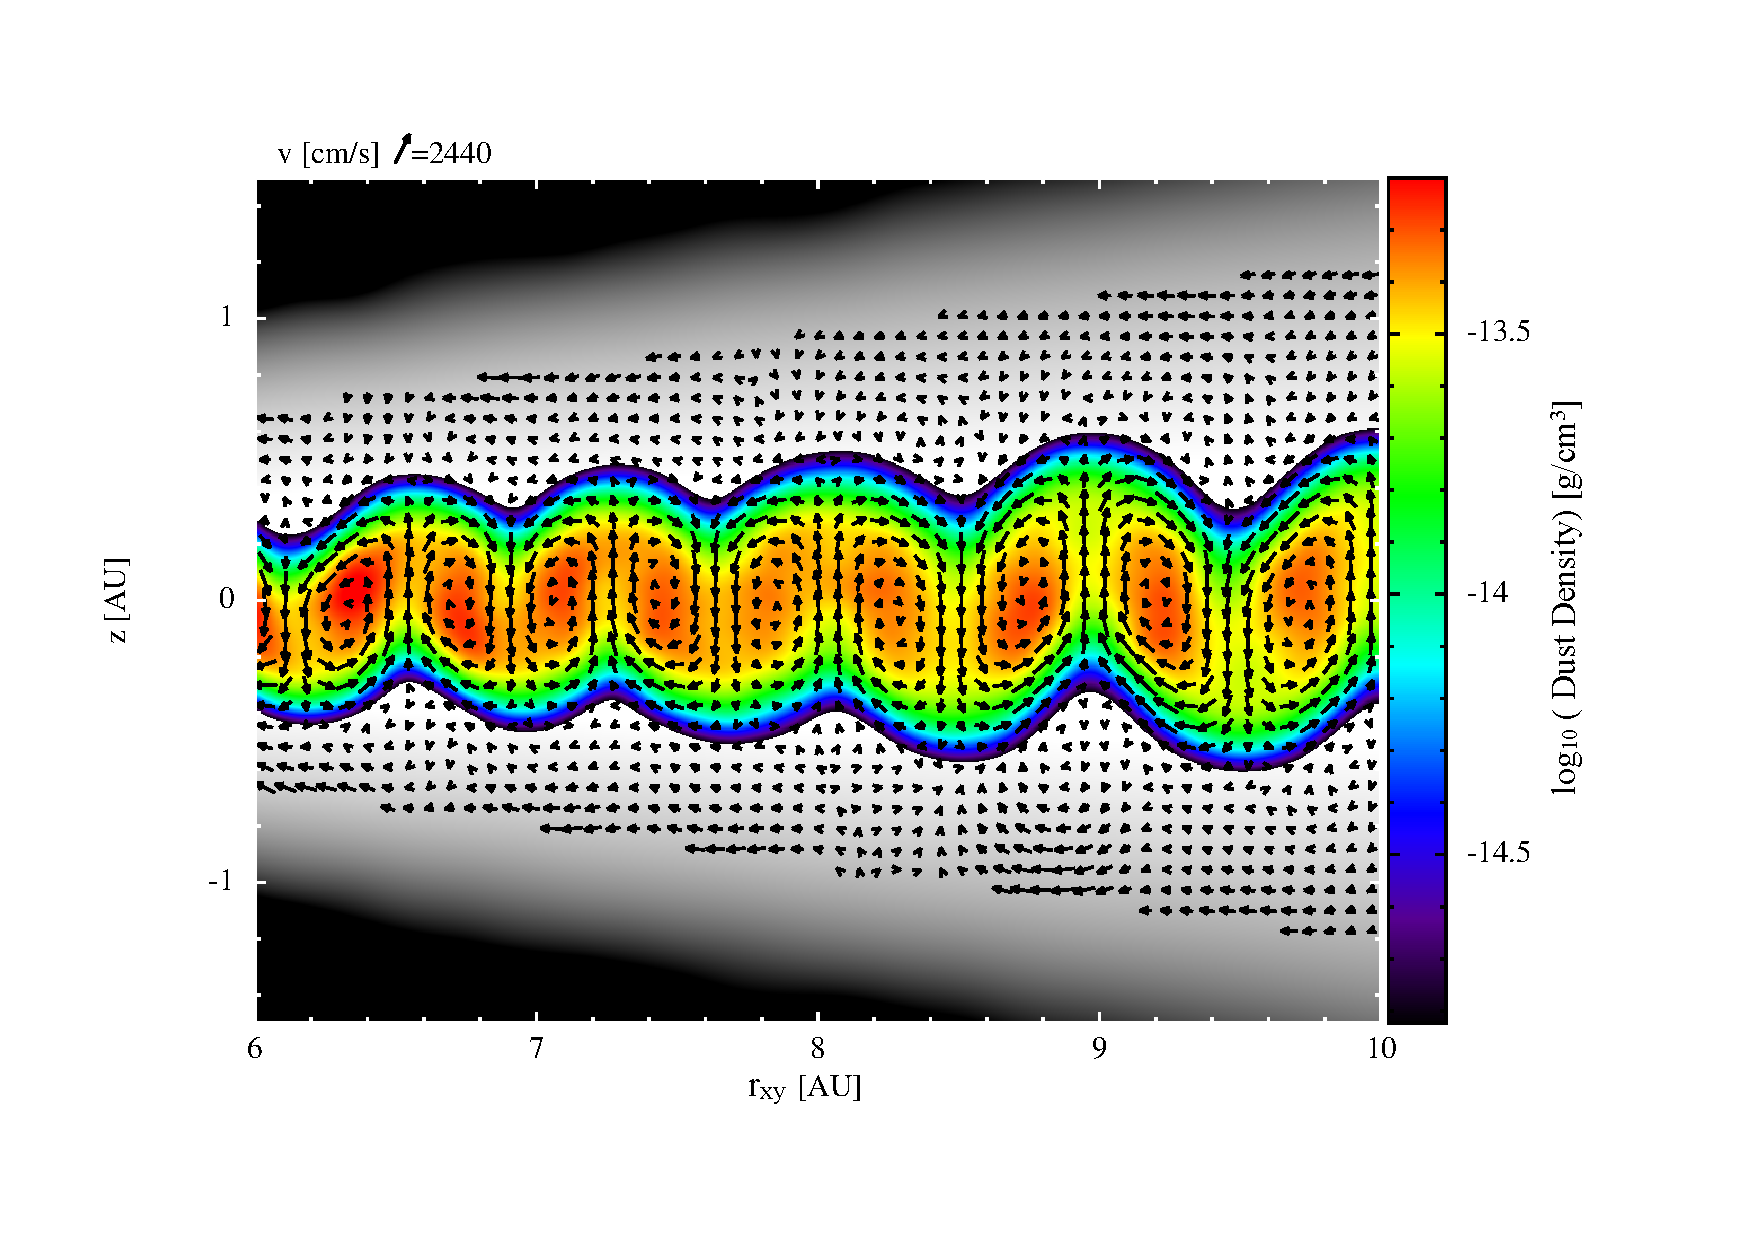
\includegraphics[scale=0.27]{figures/loren1}
      \end{center}
%    \end{minipage}
 %%   \begin{minipage}{0.39\linewidth}
    %  \begin{itemize}
     %% \item   Dusty-gas sims. from \\
        %\cite{loren15}
%      \end{itemize}
 %   \end{minipage}
 \end{itemize}
  % }
        %   \only<2>{
%     \begin{minipage}{0.6\linewidth}
%       \vspace{0.5cm}
%     \begin{center}
%       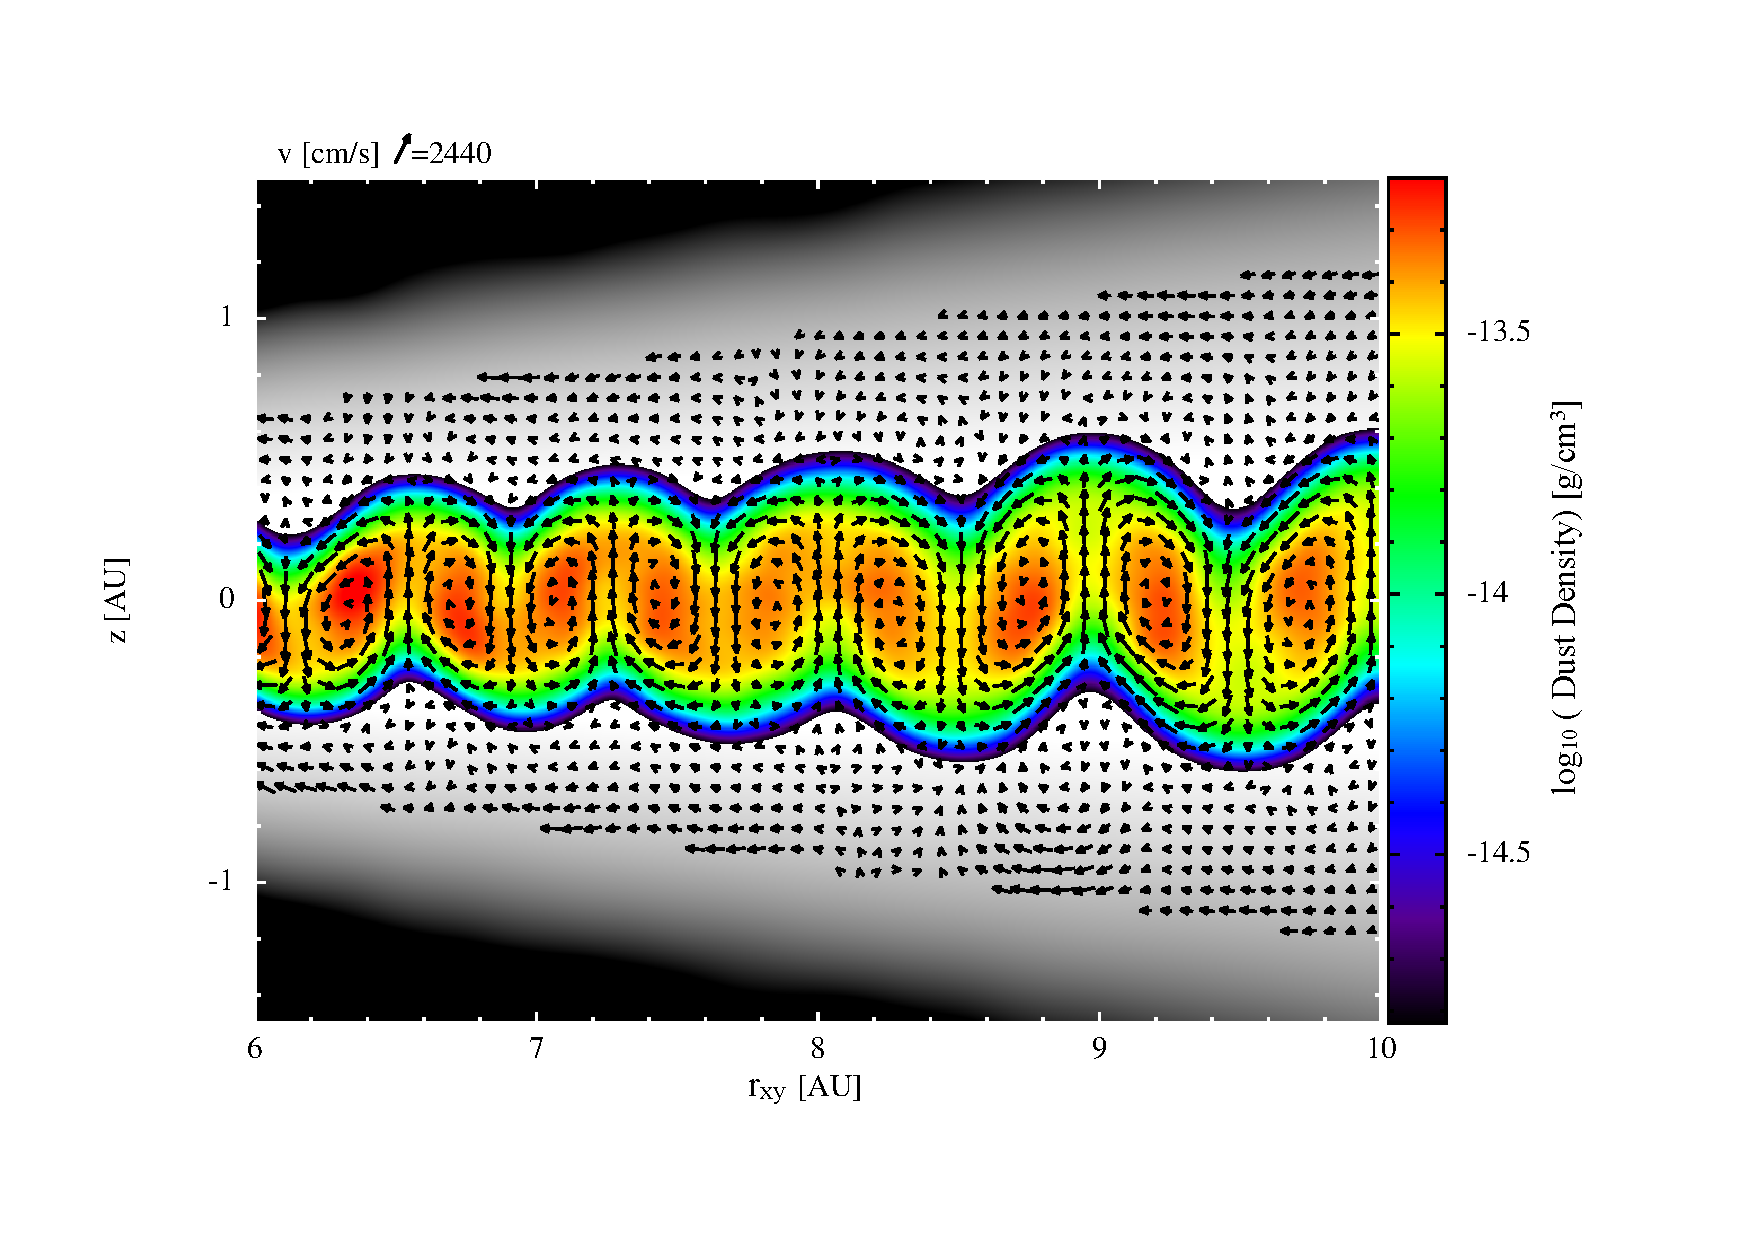
\includegraphics[scale=0.27]{figures/loren1}
%     \end{center}
%     \end{minipage}
%     \begin{minipage}{0.39\linewidth}
%       \begin{itemize}
%       \item   Dusty-gas sims. from \\
%       \cite{loren15}
%       \item What is this?
%       \end{itemize}
%     \end{minipage}
%     }
\end{frame}

% \begin{itemize}
 % \item Develop linear theory for VSI with perfectly-coupled, small dust particles
 % \item Any students interested? \textcolor{blue}{Let's talk!}
 % \end{itemize}






%----------- slide --------------------------------------------------%
\begin{frame}
  \frametitle{References}
  %% \begin{onlinebox}{12cm}
  %%  MP1303, \href{mailto:mklin924@cita.utoronto.ca}{mklin924@cita.utoronto.ca}, \href{cita.utoronto.ca/~mklin924}{cita.utoronto.ca/$\sim$mklin924}
  %% \end{onlinebox}
  \bibliographystyle{mn2e}
  \bibliography{ref}
\end{frame}


%\begin{frame}
%  \frametitle{Elliptic vortex evolution in 3D self-gravitating disks}
%  {\scriptsize or the GI of elliptical vortices}
%  \begin{figure}
%    \includegraphics[width=\linewidth]{figures/athevol_omegaz}
%  \end{figure}
%  N.B. $Q_\mathrm{3D}\equiv \frac{\Omega^2}{4\pi G \rho_\mathrm{mid}}\lesssim 0.2$ for classic GI \citep{mamat10,lin14} 
%\end{frame}

%----------- slide --------------------------------------------------%
%----------- slide --------------------------------------------------%
%% \begin{frame}
%%   \frametitle{Gravitational edge modes}
%%   \begin{figure}
%%     \centering
%%     \includegraphics[scale=.75,clip=true,trim=2.21cm 0.84cm 3.53cm 0.84cm]{figures/edge_mode.ps}
%%   \end{figure}
%% \end{frame}
\end{document}
